\section[$\etmiss$ stability over 2009 data-taking period]{$\etmissB$ stability over 2009 data-taking period}
\label{sc:METStab}

An important aspect of the MET commissioning is monitoring of the
MET-related quantities and their stability over an extended period of
time. Any instability in these quantities during stable beam conditions
can be an indication of some sort of a problem.
Figures~\ref{fig:SumET_vs_run}, \ref{fig:MET_vs_run},
\ref{fig:MEx_vs_run}, and \ref{fig:MEy_vs_run} show the stability of
several $\etmiss$-related quantities in 2009 collision data with the
HLT\_PhysicsDeclared bit set, including the ``bad'' runs listed in
Sec.~\ref{sc:DataSamples}. These types of trend plots can be used in online DQM
for monitoring the detector performance, since it can help to identify
hardware problems in calorimeter, as it is explained below.

%Fig.~\ref{fig:SumET_vs_run}-\ref{fig:MEy_vs_run} show distributions of
%various calorimetric variables versus run number for the 2009 data-taking
%period.
The trend plots clearly show that in some of the runs there
were calorimeter problems that affected measured distributions 
of $\etmiss$-related quantities. It was
confirmed by HCAL DQM that in runs 123970, 123976, 123977,
123978, 123987 the high voltages for HCAL HB and HE were off. As
a result, the total energy reconstructed in the event was lower than in
an event with fully operational HCAL, which explains the drop in
the mean of $\sumet$ and $\etmiss$ as shown on
Fig.~\ref{fig:SumET_vs_run} and \ref{fig:MET_vs_run}. 
% Run 124006, which also deviates from the trend, was identified by ECAL DQM as having an
% integrity problem in ECAL EB detector. As can be seen from
% Fig.~\ref{fig:MET_vs_run}, the mean of $\etmiss$
% distribution in this runs is higher than the average.
In run 124230 one half of the negative side of HE was not read out which
explains a slight drop in the mean $\sumet$ in Fig.~\ref{fig:SumET_vs_run}.
% During the run 123985 HCAL HB and HE, and ECAL EB and EE
% detectors were off, which can be seen in these plots as the entry
% with the smallest mean transverse energy. 
Run 124120 is the only run at $2.36$ TeV shown in the trend plots and it clearly stands out in
Figures~\ref{fig:SumET_vs_run} and \ref{fig:MET_vs_run} since collisions at higher energies
produce larger average $\sumet$ and $\etmiss$.

\begin{figure}[h!]
  \centering
  \begin{tabular}{ll}
    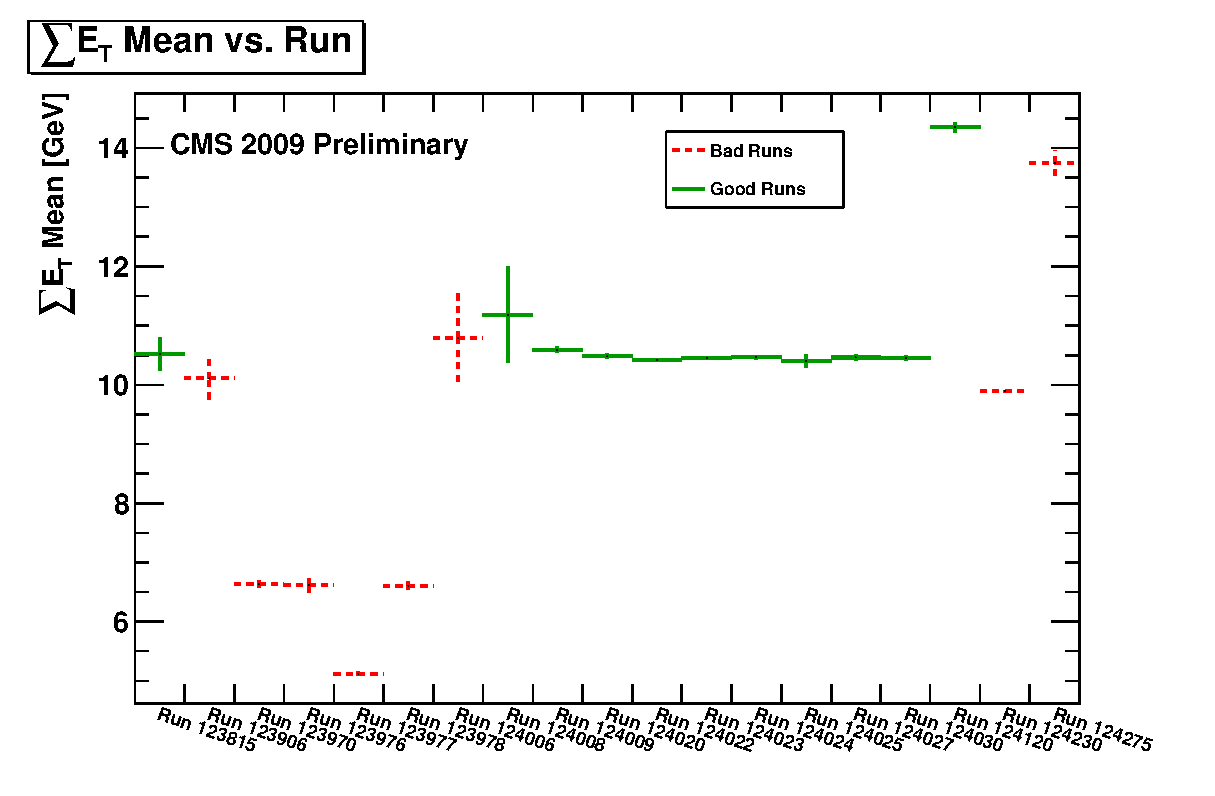
\includegraphics[width=0.5\textwidth]{plots_METStability/h_caloSumetMean_vs_run.eps} &
    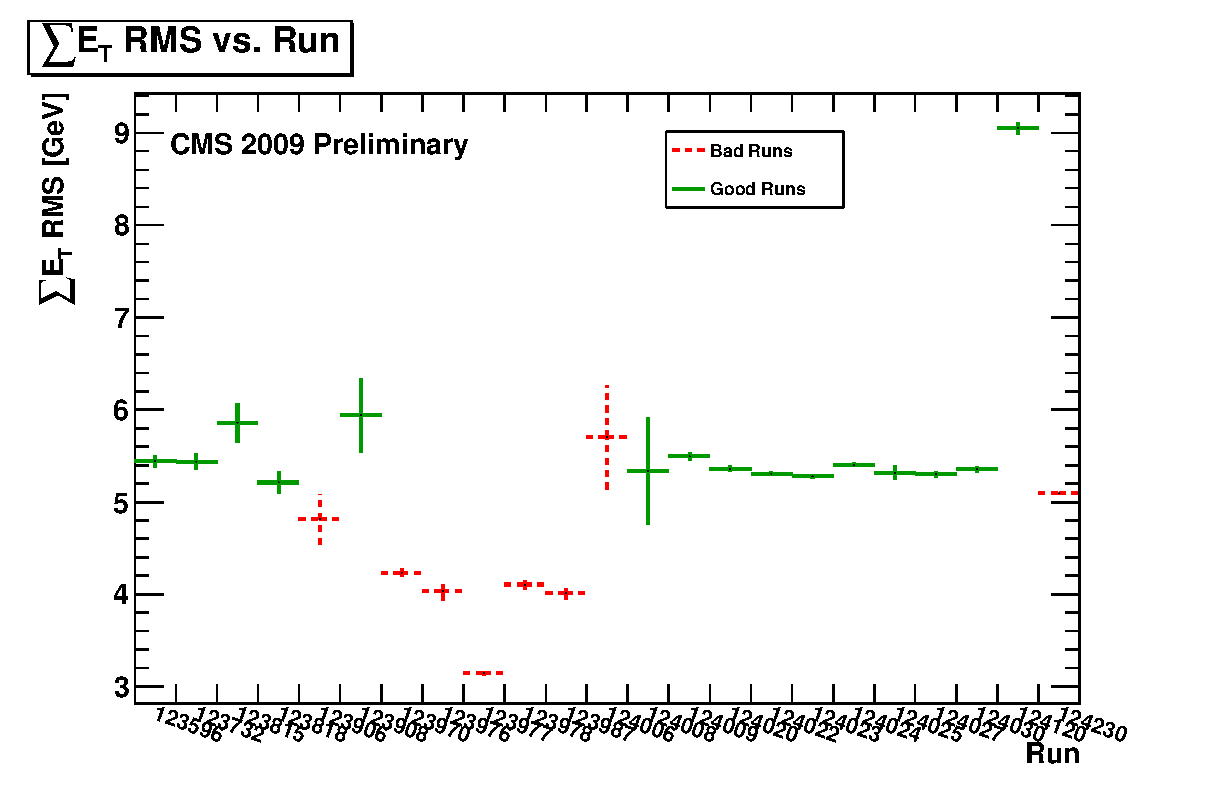
\includegraphics[width=0.5\textwidth]{plots_METStability/h_caloSumetRMS_vs_run.eps} \\
  \end{tabular}
 \caption{\small The mean and RMS of the $\sumet$ distribution vs. run number for the 2009 data-taking period.
          Entries shown in red correspond to runs with some known hardware problems. Run 124120 is a $2360$ GeV run.
          \label{fig:SumET_vs_run}}
      \end{figure}

\begin{figure}[h!]
  \centering
  \begin{tabular}{ll}
    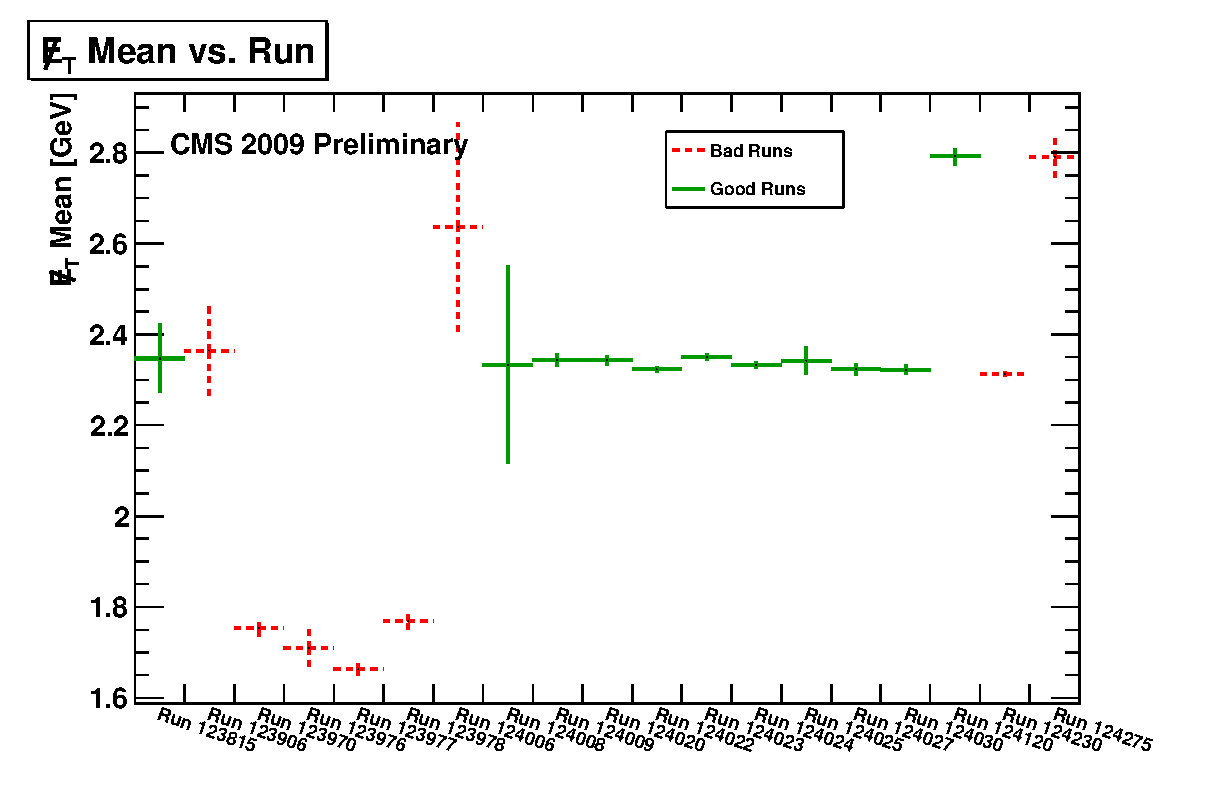
\includegraphics[width=0.5\textwidth]{plots_METStability/h_calometPtMean_vs_run.eps} &
    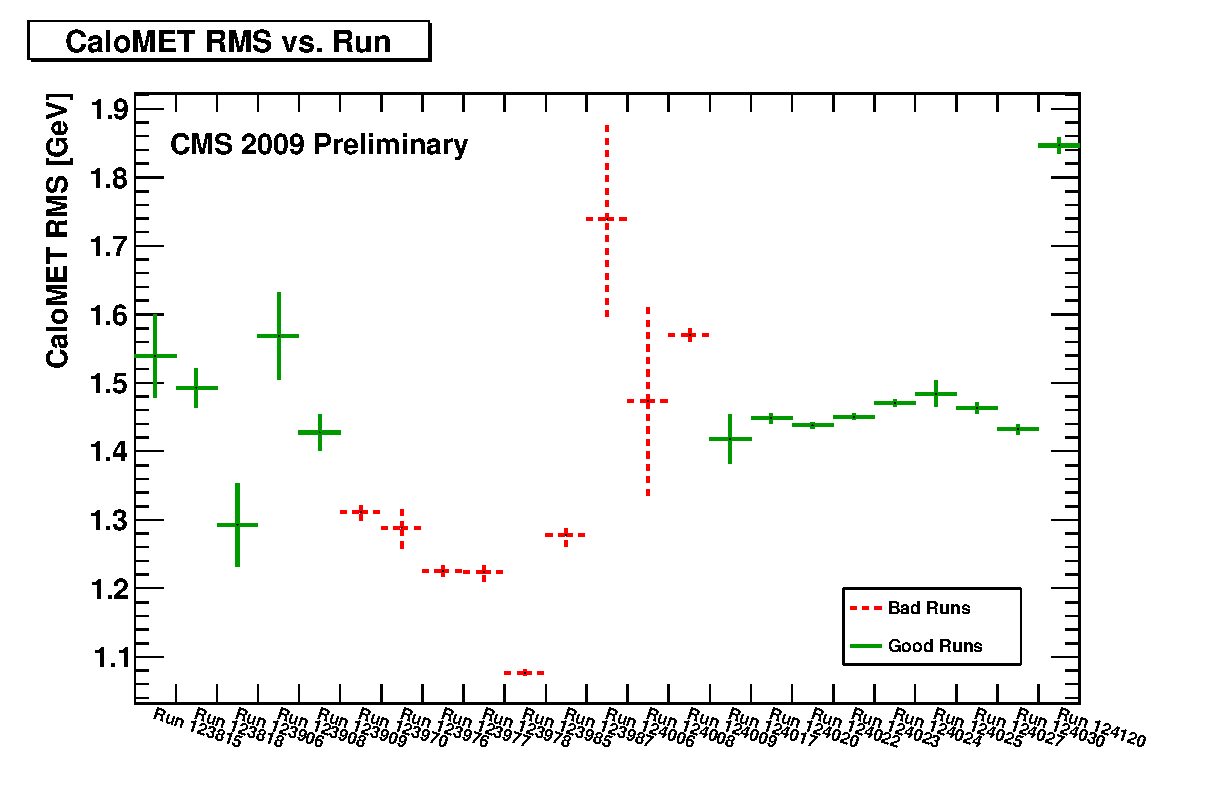
\includegraphics[width=0.5\textwidth]{plots_METStability/h_calometPtRMS_vs_run.eps} \\
  \end{tabular}
  \caption{\small The mean and RMS of the $\etmiss$ distribution vs. run
    number for the 2009 data-taking period.  Entries shown in red
    correspond to runs with some known hardware problems. Run 124120 is a $2360$ GeV run.\label{fig:MET_vs_run}}
\end{figure}

Monitoring the $x$ and $y$ components of $\etmiss$ can be helpful in
identifying any asymmetric behaviour in the
calorimeters. In Fig.~\ref{fig:MEx_vs_run} one can see a flat
distribution in $\exmiss$ indicating an expected behaviour. The
distribution of $\sigma\left(\exmiss\right)$ drops during the runs with parts of
detector off, which is expected since the $\sigma\left(\exmiss\right)$ is
proportional to $\sumet$. 
% However, the mean of the $\eymiss$ distribution on
% Fig.~\ref{fig:MEy_vs_run} shows a drop during runs with HB and HE off,
% which may indicate that there is some asymmetry in the response of the
% ECAL calorimeter.

\begin{figure}[h!]
  \centering
  \begin{tabular}{ll}
    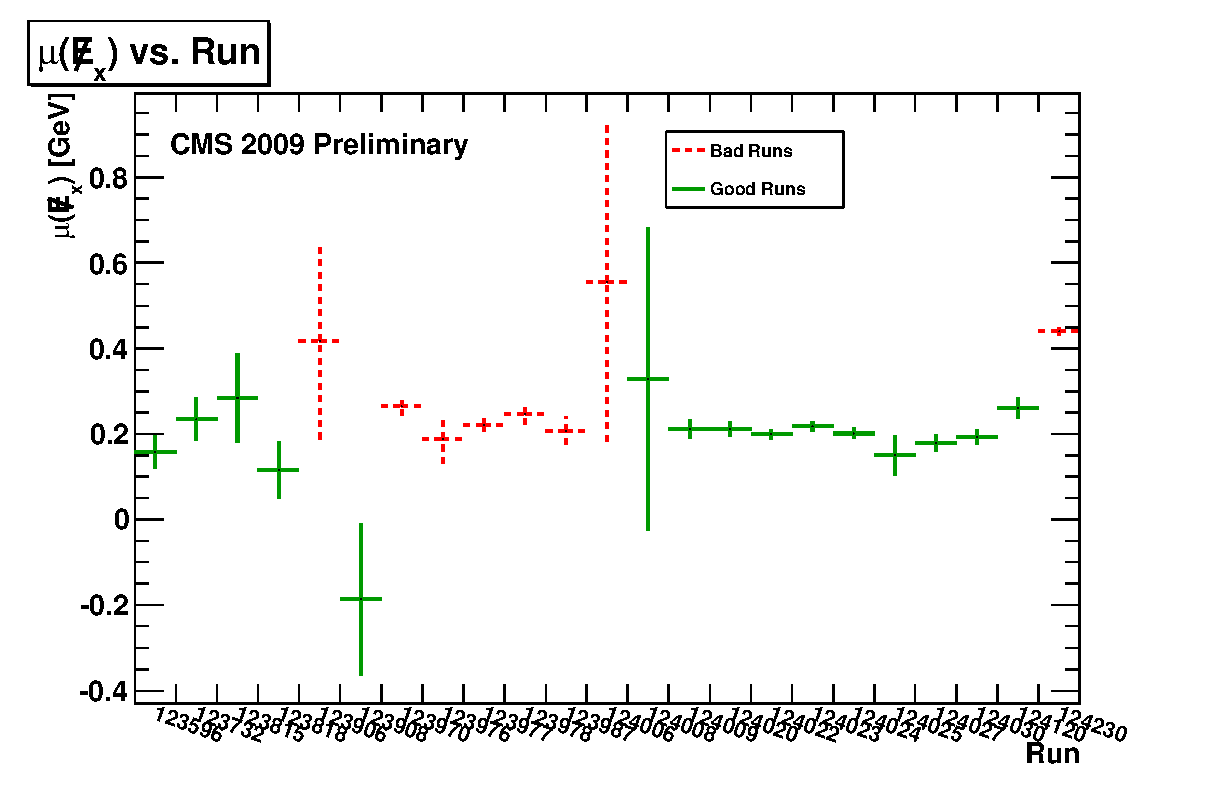
\includegraphics[width=0.5\textwidth]{plots_METStability/h_calometPxMean_vs_run.eps} &
    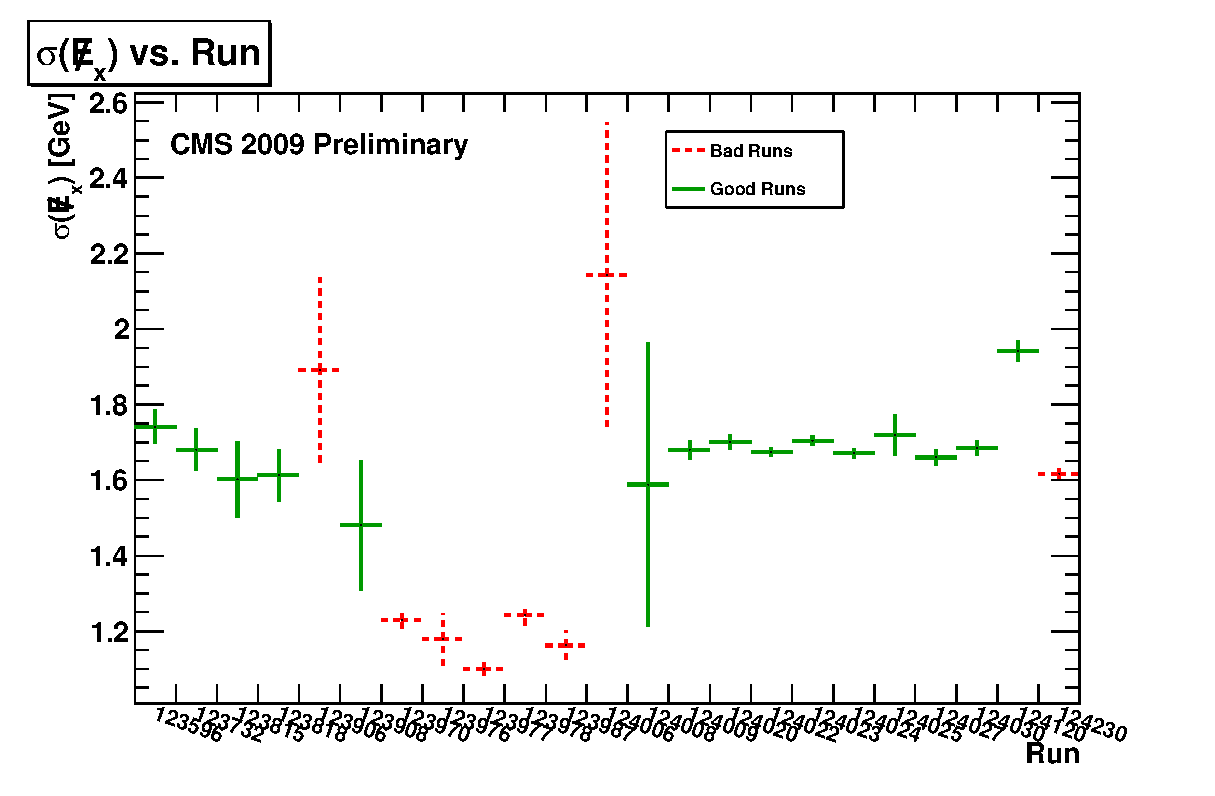
\includegraphics[width=0.5\textwidth]{plots_METStability/h_calometPxSigma_vs_run.eps} \\
  \end{tabular}
  \caption{\small The mean and $\sigma$ of the $\exmiss$ distribution
    vs. run number for the 2009 data-taking period.  Entries shown in
    red correspond to runs with some known hardware problems. Run 124120 is a $2360$ GeV run.\label{fig:MEx_vs_run}}
\end{figure}

\begin{figure}[h!]
  \centering
  \begin{tabular}{ll}
    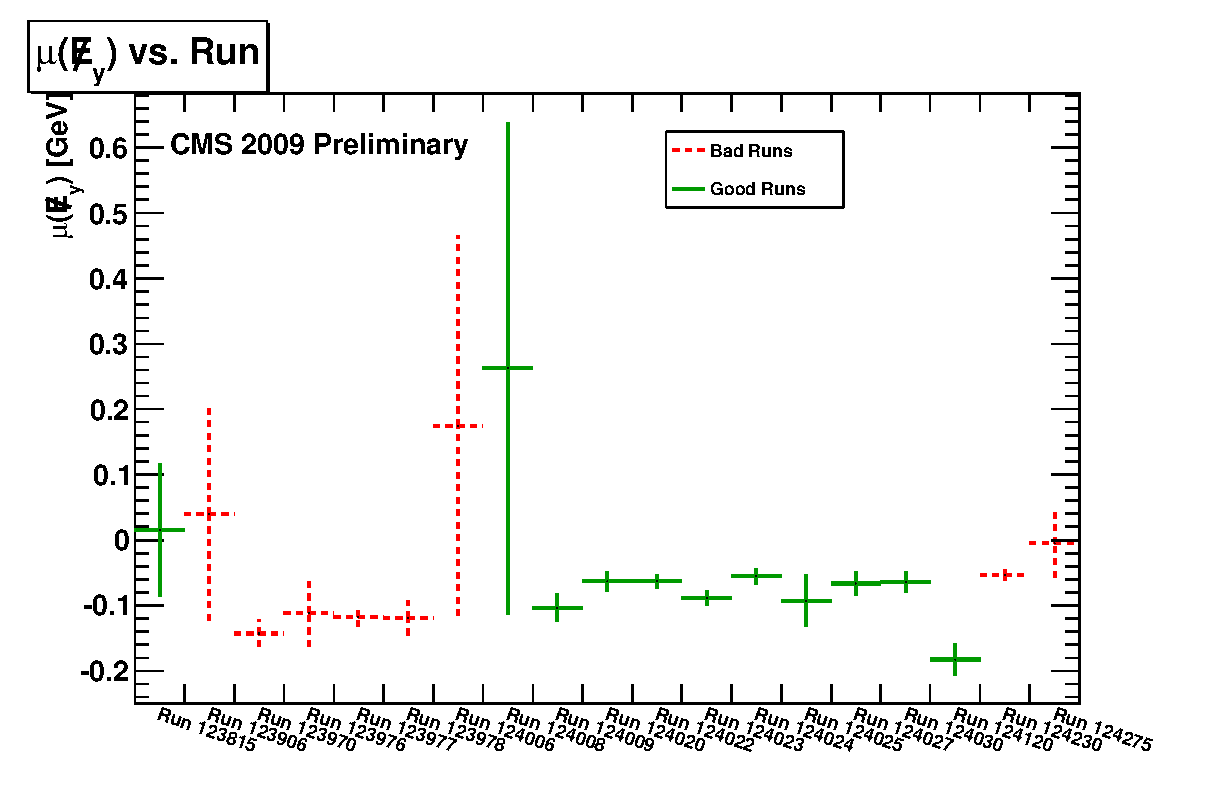
\includegraphics[width=0.5\textwidth]{plots_METStability/h_calometPyMean_vs_run.eps} &
    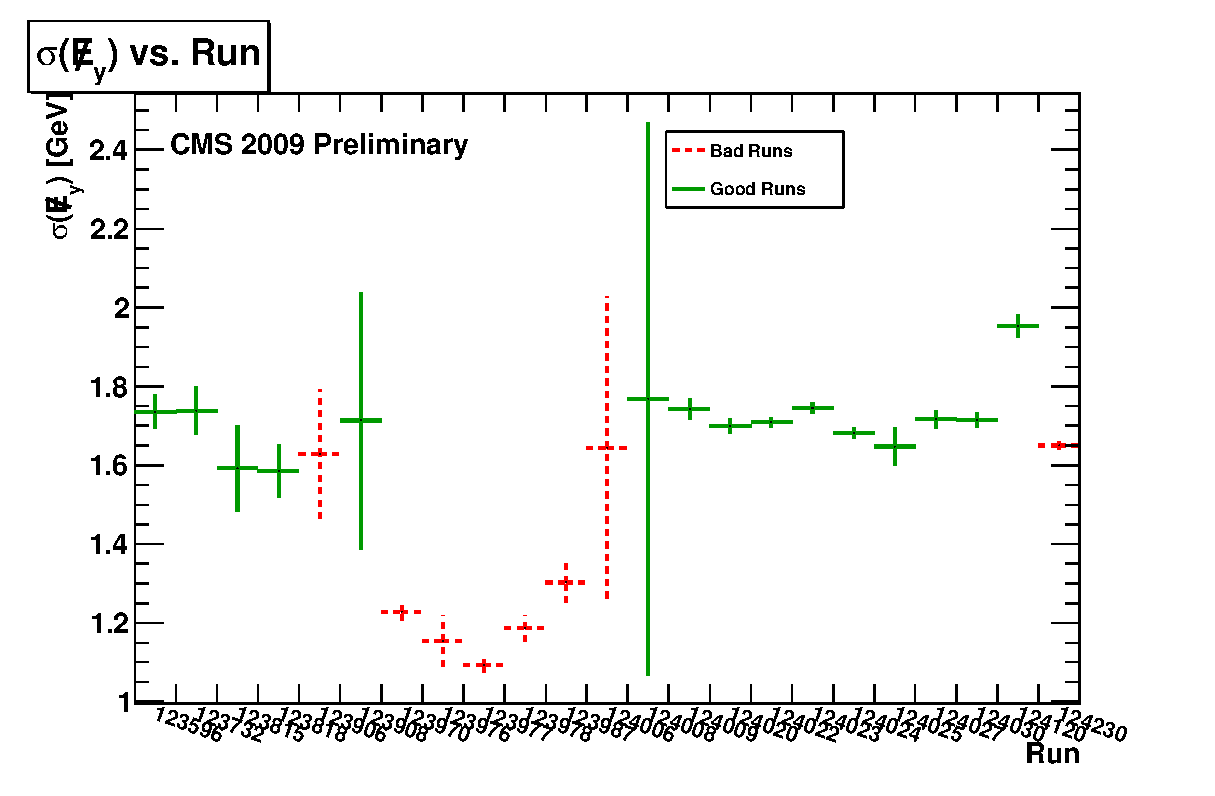
\includegraphics[width=0.5\textwidth]{plots_METStability/h_calometPySigma_vs_run.eps} \\
  \end{tabular}
  \caption{\small The mean and $\sigma$ of the $\eymiss$ distribution
    vs. run number for the 2009 data-taking period.  Entries shown in
    red correspond to runs with some known hardware problems. Run 124120 is a $2360$ GeV run.\label{fig:MEy_vs_run}}
\end{figure}


\clearpage

